\chapter{Interfaccia del file system}

\section{Introduzione al File System}

\begin{itemize}
    \item Il File System rappresenta la parte più visibile del Sistema Operativo per gli utenti.
    \item Fornisce i meccanismi per memorizzare e accedere ai dati e agli applicativi.
    \item Un File System è composto da:
    \begin{itemize}
        \item \textbf{Un insieme di file:} Unità logiche di informazione.
        \item \textbf{Una struttura di directory:} Permette l'organizzazione e la gestione dei file.
    \end{itemize}
\end{itemize}

\section{Concetto di File}

\dfn{File}{
    Un'unità logica di informazione memorizzata su un supporto di memoria secondaria. Caratteristiche principali:
    \begin{itemize}
        \item \textbf{Nome:} Identificativo simbolico del file.
        \item \textbf{Posizione logica:} Localizzazione nel File System.
        \item \textbf{Attributi:} Informazioni aggiuntive come dimensioni, diritti di accesso, date di creazione, accesso e modifica etc...
    \end{itemize}
}

\nt{In unix esistono 4 tipi di file: Pipe, synbolic link, block special file, character special file.}

\begin{itemize}
    \item I file possono contenere:
    \begin{itemize}
        \item \textbf{Dati:} Numerici, caratteri, binari.
        \item \textbf{Programmi:} Sorgenti, linkabili, eseguibili.
        \item \textbf{Documenti:} Multimediali o omogenei.
    \end{itemize}
    \item La struttura interna dei file dipende dal tipo:
    \begin{itemize}
        \item File di testo: Caratteri organizzati in righe.
        \item Programmi sorgenti: Suddivisi in procedure e dati.
        \item File eseguibili: Suddivisi in segmenti.
    \end{itemize}
    \item In ultima analisi, un file è una semplice sequenza di bit.
\end{itemize}

\subsection{Attributi dei File}

Ogni file è associato a una serie di attributi utili per gestirne l'uso e le operazioni:

\begin{itemize}
    \item \textbf{Nome simbolico:} Adeguato per l'uso umano.
    \item \textbf{Tipo:} Specifico per sistemi operativi che distinguono tra diversi tipi di file.
    \item \textbf{Posizione fisica:} Localizzazione sul supporto di memoria secondaria.
    \item \textbf{Posizione logica:} Il \textit{pathname} che individua il file all'interno del File System.
    \begin{itemize}
        \item Nota: Questa informazione fondamentale non è sempre memorizzata esplicitamente, tranne in alcuni casi particolari.
    \end{itemize}
    \item \textbf{Dimensione corrente:} 
    \begin{itemize}
        \item La dimensione effettiva del file può variare rispetto allo spazio che occupa in memoria secondaria.
        \item Caso raro: Un file può occupare meno spazio in memoria a causa di tecniche di compressione o struttura.
    \end{itemize}
\end{itemize}

Gli attributi di un file includono informazioni cruciali per la gestione e la protezione dei dati:

\begin{itemize}
    \item \textbf{Permessi di accesso/Protezione:} Controllano chi può leggere, scrivere o eseguire un file, proteggendolo da accessi non autorizzati.
    \item \textbf{Data e ora:} Include informazioni sulla creazione, ultima modifica e ultimo accesso al file.
    \item \textbf{Identificazione del proprietario:} Specifica l'utente proprietario, fondamentale per sistemi multiutente.
    \item \textbf{Memorizzazione:} Gli attributi possono occupare anche più di un \textbf{kilobyte di memoria secondaria}. Sono memorizzati in strutture dati accessibili attraverso il sistema di directory.
\end{itemize}

\subsection{Operazioni sui File}

Un file può essere visto come un tipo di dato astratto, le cui operazioni principali includono:

\begin{itemize}
    \item \textbf{Creazione:} Richiede al Sistema Operativo di allocare spazio e creare un riferimento al file nella directory.
    \item \textbf{Scrittura/Lettura:}
    \begin{itemize}
        \item Il Sistema Operativo gestisce il puntatore di lettura/scrittura.
        \item Garantisce spazio sufficiente per l'espansione del file in caso di scrittura.
    \end{itemize}
    \item \textbf{Riposizionamento:} Permette di modificare la posizione del puntatore per leggere o scrivere a partire da un punto specifico.
    \item \textbf{Rimozione:} Libera lo spazio occupato dal file sia sul disco che nella directory.
    \item \textbf{Troncamento:} Cancella i dati ma mantiene gli attributi del file.
    \item \textbf{Altre operazioni:}
    \begin{itemize}
        \item Rinominare il file.
        \item Copiare il contenuto in un altro file.
        \item Spostare il file tra directory.
    \end{itemize}
\end{itemize}

\subsection{Metodi d’Accesso ai File}

\begin{itemize}
    \item \textbf{Accesso sequenziale:} I dati vengono letti o modificati in ordine, partendo dall’inizio del file.
    \item \textbf{Accesso diretto:} Permette di accedere a un punto specifico del file, ad esempio per leggere la millesima riga di un testo.
    \begin{itemize}
        \item L'accesso diretto può essere simulato da quello sequenziale, ma risulta inefficiente.
        \item I metodi di allocazione dei file influiscono sull'efficienza dell'accesso diretto.
    \end{itemize}
\end{itemize}

\section{Struttura delle Directory (o cartelle, o folder)}
\label{sec:directory_structure}

Un File System (FS) può essere molto grande, arrivando a contenere decine di migliaia di file e occupare centinaia di gigabyte. Di conseguenza, è necessaria un'organizzazione che consenta di accedere a questi dati in tempi ragionevoli.

\clm{}{}{
    È fondamentale che i tempi di accesso ai singoli file (dati e attributi) non crescano linearmente con il numero di file o lo spazio occupato.
}

\subsection{Directory e gestione dei file}
Un sistema di directory è utilizzato per tenere traccia dei file di un FS e organizzarli in modo conveniente. Una directory “contiene” i file, consentendo di risalire a tutte le informazioni relative a ciascun file (dati e attributi) a partire dal suo nome.

\subsection{Informazioni recuperabili dalle directory}
Per ciascun file contenuto in una directory, è necessario poter recuperare alcune informazioni fondamentali, tra cui:
\begin{itemize}
    \item Posizione del file in memoria secondaria.
    \item Dimensioni correnti del file.
    \item Data dell’ultimo accesso e dell’ultima modifica.
    \item ID del proprietario del file.
    \item Protezioni e permessi di accesso.
\end{itemize}

\subsection{Operazioni sulle directory}
Le directory supportano diverse operazioni fondamentali, come:
\begin{itemize}
    \item Ricerca di un file.
    \item Creazione o cancellazione di un file.
    \item Visualizzazione del contenuto della directory.
    \item Cambiamento del nome di un file.
    \item Spostamento di un file in un’altra directory.
\end{itemize}

Le informazioni contenute nella directory sono essenziali per l’accesso ai file. \textbf{Perdere i dati della directory comporta quasi sempre la perdita di accesso ai file stessi.}

\subsection{Struttura delle directory}
Le directory, tecnicamente, sono dei file speciali che contengono informazioni su altri file (quelli “contenuti” nella directory stessa). Un file directory è strutturato in un certo numero di \textit{entry}, una per ogni file contenuto, dove ogni entry può includere:
\begin{itemize}
    \item Il nome del file.
    \item Attributi del file.
    \item Un puntatore a una struttura che contiene ulteriori dettagli.
\end{itemize}

Tuttavia, a differenza degli altri file, una directory non può essere modificata liberamente dal suo possessore. Le modifiche devono essere effettuate tramite le operazioni messe a disposizione dal sistema operativo, che garantisce l’integrità della struttura della directory. In caso contrario, i file contenuti e i loro attributi potrebbero diventare irrecuperabili.

\subsection{Le directory in MS-DOS}
In MS-DOS, ogni file nella directory è accompagnato da informazioni quali attributi (dimensioni, data di creazione/accesso, tipo, ecc.) e posizione sul supporto di memoria secondaria. Un esempio di directory in MS-DOS:
\begin{verbatim}
lista.txt   attributi vari
nomi.doc    attributi vari
prog.c      attributi vari
quake       attributi vari
\end{verbatim}

In ms-dos un file directory è (era) fatto di una serie di entry di 32 byte ciascuna, dove ogni entry contiene:
\begin{figure}[h] \centering 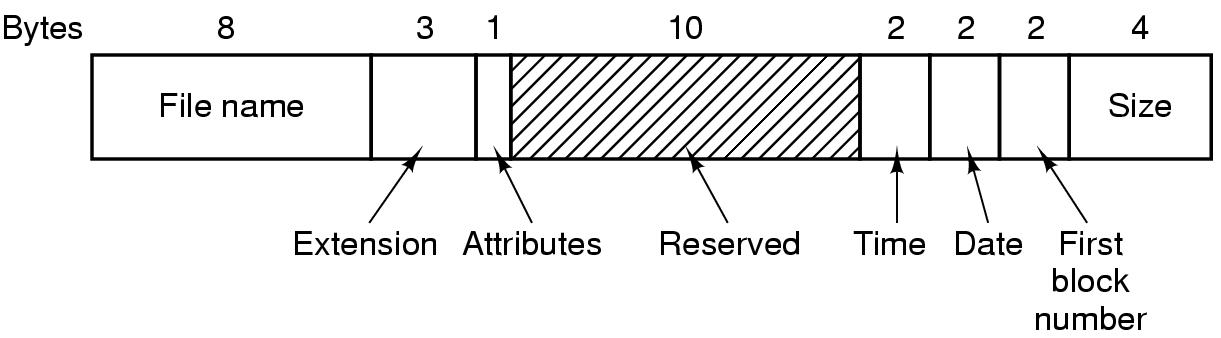
\includegraphics[width=0.50\linewidth]{images/entry_msDos_dir.png} \caption{Entry directory ms-dos} \end{figure}

\subsection{Le Directory in Unix}
Nei sistemi Unix-like, invece di memorizzare direttamente gli attributi di un file all’interno della directory, accanto al nome di ciascun file viene inserito un puntatore a una struttura interna, gestita direttamente dal sistema operativo e memorizzata in memoria secondaria. Questa struttura contiene tutte le informazioni sul file.

\subsection{Le Directory in NTFS}
\nt{
    Nei file system più moderni, come NTFS (New Technology File System), adottato a partire da Windows XP, sono possibili soluzioni alternative e combinate.
}
In NTFS, le entry delle directory non sono organizzate in modo lineare, come accadeva in MS-DOS, ma utilizzano una struttura ad **albero di ricerca bilanciato**. In questa struttura, ogni foglia dell’albero rappresenta un file contenuto nella directory. 

\clm{Vantaggi}{}{
    Grazie alla struttura ad albero bilanciato:
    \begin{itemize}
        \item Il tempo necessario per accedere alle informazioni di un file è costante, indipendentemente dalla posizione del file all’interno della directory.
    \end{itemize}
}

Ogni foglia dell’albero di ricerca contiene:
\begin{itemize}
    \item Il nome del file.
    \item Un puntatore (detto \textit{file reference}) a una struttura interna memorizzata in memoria secondaria, che contiene tutte le informazioni associate al file.
    \item Alcuni attributi del file, come la dimensione corrente e la data dell’ultimo aggiornamento, replicati nella foglia per ragioni di efficienza.
\end{itemize}

\subsection{Directory ad un solo livello}
La soluzione più semplice per organizzare i file in un FS è mediante una directory unica che contiene tutti i file (Fig. 13.7). 

\wc{Soluzione adatta per sistemi complessi}{
    Questa organizzazione è facile da implementare, ma presenta notevoli svantaggi:
    \begin{itemize}
        \item Non consente a utenti diversi di avere file con lo stesso nome.
        \item Non permette di raggruppare separatamente i file.
        \item La ricerca di un file può risultare inefficiente.
    \end{itemize}
}

\begin{figure}[h] \centering 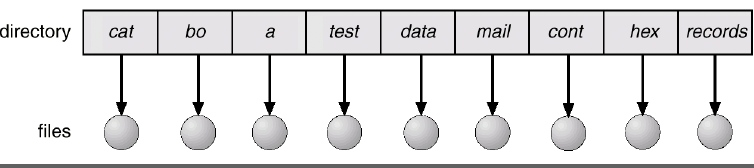
\includegraphics[width=0.50\linewidth]{images/dir_singleLevel.png} \caption{Directory a singolo livello} \end{figure}

\subsection{Directory a due livelli}
Un miglioramento rispetto alla soluzione precedente è rappresentato da una struttura a due livelli. In questo caso, esiste una directory principale che contiene le directory di ciascun utente (Fig. 13.8). 

\clm{Vantaggi}{}{
    \begin{itemize}
        \item I file di utenti diversi sono raggruppati separatamente, migliorando l’organizzazione.
        \item La ricerca dei file diventa più efficiente.
    \end{itemize}
}
Tuttavia, i file di ciascun utente sono ancora tutti raggruppati nella stessa directory personale.

\begin{figure}[h] \centering 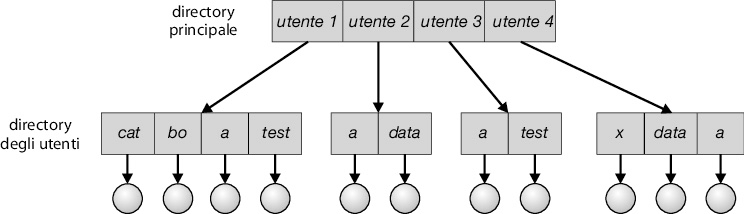
\includegraphics[width=0.50\linewidth]{images/dir_doubleLevel.png} \caption{Directory a doppio livello} \end{figure}

\subsection{Directory con struttura ad albero}
Un’estensione naturale della struttura a due livelli è rappresentata dalle **directory ad albero**. In questo modello, ogni directory può contenere:
\begin{itemize}
    \item File normali.
    \item Altre directory.
\end{itemize}

Questa organizzazione è ricorsiva e permette una gerarchia arbitraria di directory e file.

\begin{figure}[h] \centering 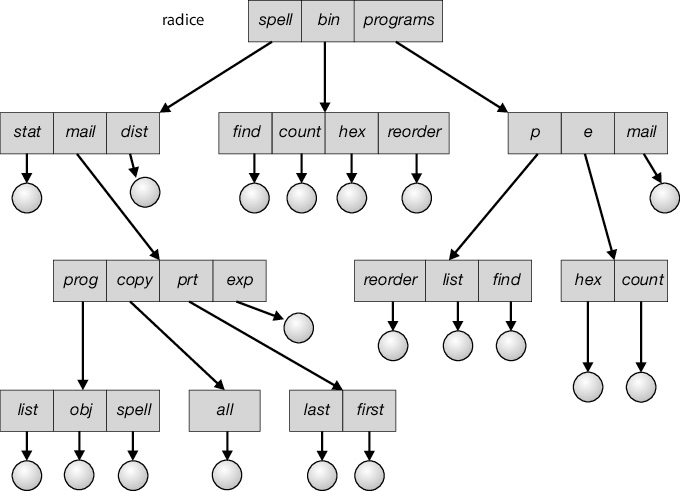
\includegraphics[width=0.50\linewidth]{images/dir_treeLevel.png} \caption{Directory con struttura ad albero} \end{figure}

\subsection{La Root e le Directory Utente}
La directory da cui si dirama l'intero File System è chiamata \textbf{Root} o radice del File System. Ogni utente ha a disposizione una porzione del File System, modellabile a piacere, che si dirama dalla propria \textbf{Home Directory}. 

\nt{
    Quando un utente avvia una sessione, viene automaticamente posizionato nella propria home directory.
}

\subsection{Navigazione e Directory Corrente}
Gli utenti possono navigare liberamente all'interno del proprio File System utilizzando comandi come \texttt{cd} o l'interfaccia grafica. Durante l'utilizzo, ogni utente è sempre "posizionato" su una directory specifica, detta \textbf{current directory} o \textbf{working directory}. 

\qs{Esempio di current directory}{
    Qual è la current directory in un sistema con interfaccia a finestre?
}

A fianco del \textbf{pathname assoluto}, definito a partire dalla radice del File System, emerge il concetto di \textbf{pathname relativo}, che è definito rispetto alla current directory.

\subsection{Pathname Assoluti}
Un pathname assoluto inizia sempre con la radice del File System, indicata con un carattere speciale:
\begin{itemize}
    \item \texttt{/} (slash) per i sistemi Unix.
    \item \texttt{\textbackslash} (backslash) per i sistemi MS-DOS/Windows.
\end{itemize}

In MS-DOS/Windows, il pathname assoluto può includere il nome del volume, come \texttt{C:} o \texttt{A:}.

\ex{Esempi di pathname assoluti}{
    \begin{itemize}
        \item Unix: \texttt{/users/st123456/prog.c}
        \item MS-DOS/Windows: \texttt{C:\textbackslash users\textbackslash st123456\textbackslash prog.c}
    \end{itemize}
}

\subsection{Pathname Relativi}
Un pathname relativo non inizia con \texttt{/} o \texttt{\textbackslash}, ma con il nome di una directory rispetto alla current directory. 

\clm{Convenzioni universali}{}{
    \begin{itemize}
        \item \texttt{.} (punto) rappresenta la current directory.
        \item \texttt{..} (punto punto) rappresenta la parent directory (directory genitrice).
    \end{itemize}
}

\ex{Esempi di pathname relativi}{
    \begin{itemize}
        \item \texttt{bin/gcc}: file \texttt{gcc} nella sottodirectory \texttt{bin}.
        \item \texttt{../prog.c}: file \texttt{prog.c} nella parent directory.
        \item \texttt{../users/st123456/prog.c}: percorso relativo partendo dalla current directory.
    \end{itemize}
}

\subsection{Utilizzo dei Pathname}
Il pathname, sia relativo che assoluto, può essere utilizzato come argomento di comandi o system call. Esempi in Unix:
\begin{itemize}
    \item \texttt{ls -l ../users/st13456/prog.c}
    \item \texttt{fopen("/users/st13456/prog.c", "w");}
\end{itemize}

\nt{
    Anche nei sistemi a finestre, un eseguibile che opera su un file deve comunque fare riferimento al file attraverso il suo pathname.
}

\subsection{Comandi per la Gestione delle Directory}
La presenza di directory e sottodirectory richiede comandi adeguati per la gestione del File System, come:
\begin{itemize}
    \item \texttt{mkdir [pathname]nomedir}: crea una nuova directory.
    \item \texttt{rmdir [pathname]nomedir}: rimuove una directory.
    \item \texttt{cd pathname}: riposiziona la current directory su \texttt{pathname}.
\end{itemize}

\nt{
    Nelle interfacce a finestre, operazioni analoghe possono essere effettuate tramite menu, ma in ogni caso tali operazioni sono implementate attraverso system call.
}

\subsection{Directory con Struttura a Grafo Aciclico}
La struttura ad albero presenta una limitazione significativa: non permette di condividere file o directory con nomi diversi. Questo limita la condivisione e la cooperazione, in quanto uno stesso file non può essere visto da directory diverse usando nomi differenti. 

\clm{Concetto di Link}{}{
    I diversi collegamenti ad un file o directory vengono chiamati \textbf{link}. Questi possono essere implementati in modi diversi nei vari sistemi operativi, ottenendo risultati differenti.
}

\nt{
    La gestione dei link sarà trattata in dettaglio nel capitolo 14.
}
\begin{figure}[h] \centering 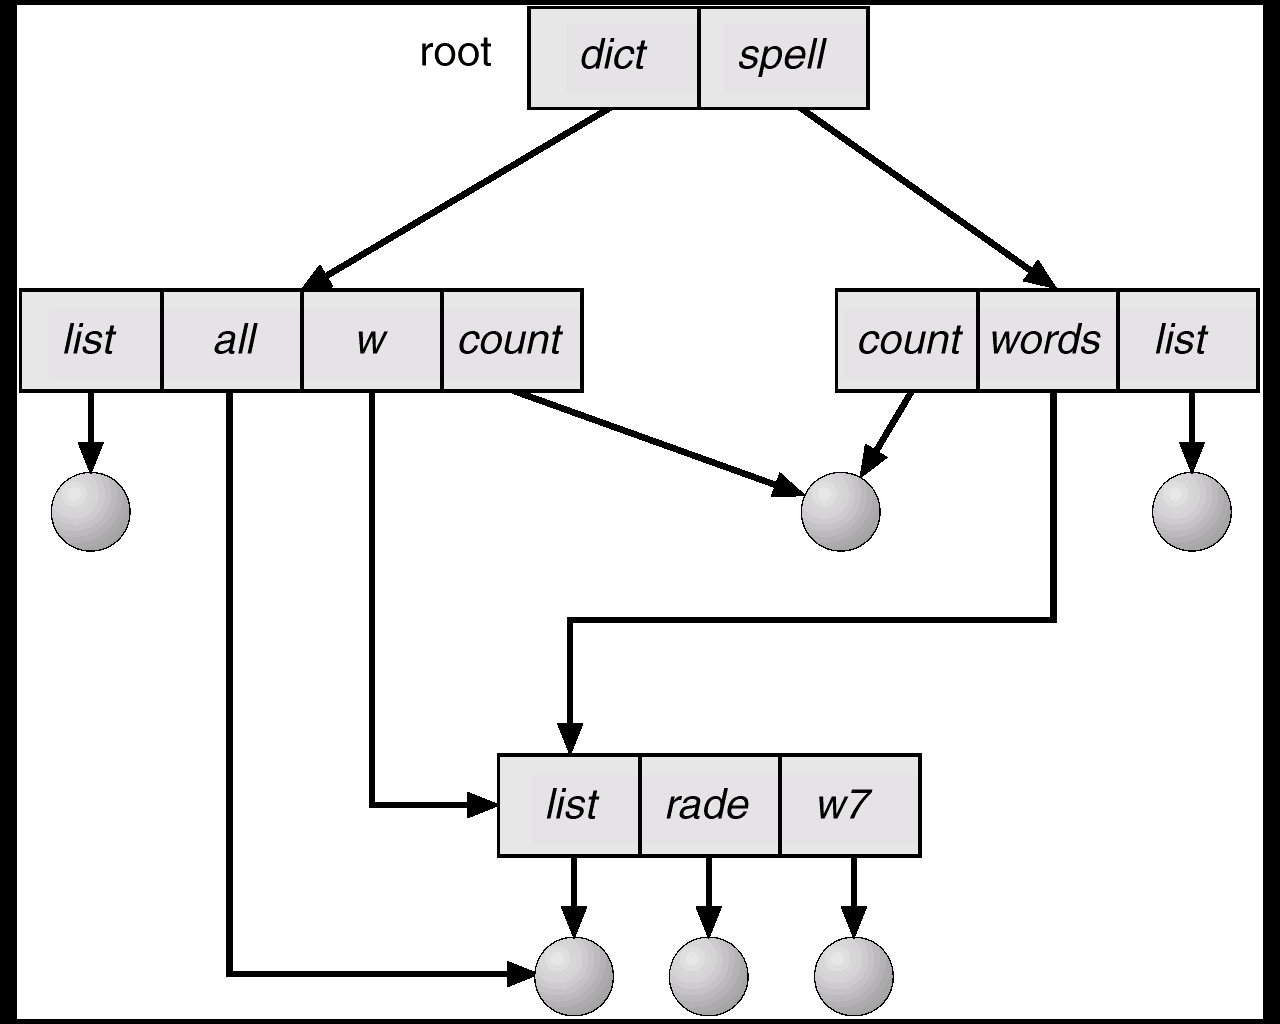
\includegraphics[width=0.50\linewidth]{images/dir_graphLevel.png} \caption{Directory con struttura a grafo aciclico} \end{figure}

\subsection{Directory con Struttura a Grafo Generale}
In un File System con una struttura a grafo generale, una directory può "contenere" il nome di una directory padre o persino di una directory antenata. Tuttavia, ciò introduce potenziali problemi:
\begin{itemize}
    \item \textbf{Cicli}: Se un programma visita ricorsivamente una directory e le sue sottodirectory, potrebbe entrare in un loop senza accorgersene.
    \item \textbf{Cancellazione}: Cosa accadrebbe se tentassimo di eliminare una directory che contiene la sua directory padre?
\end{itemize}

\begin{figure}[h] \centering 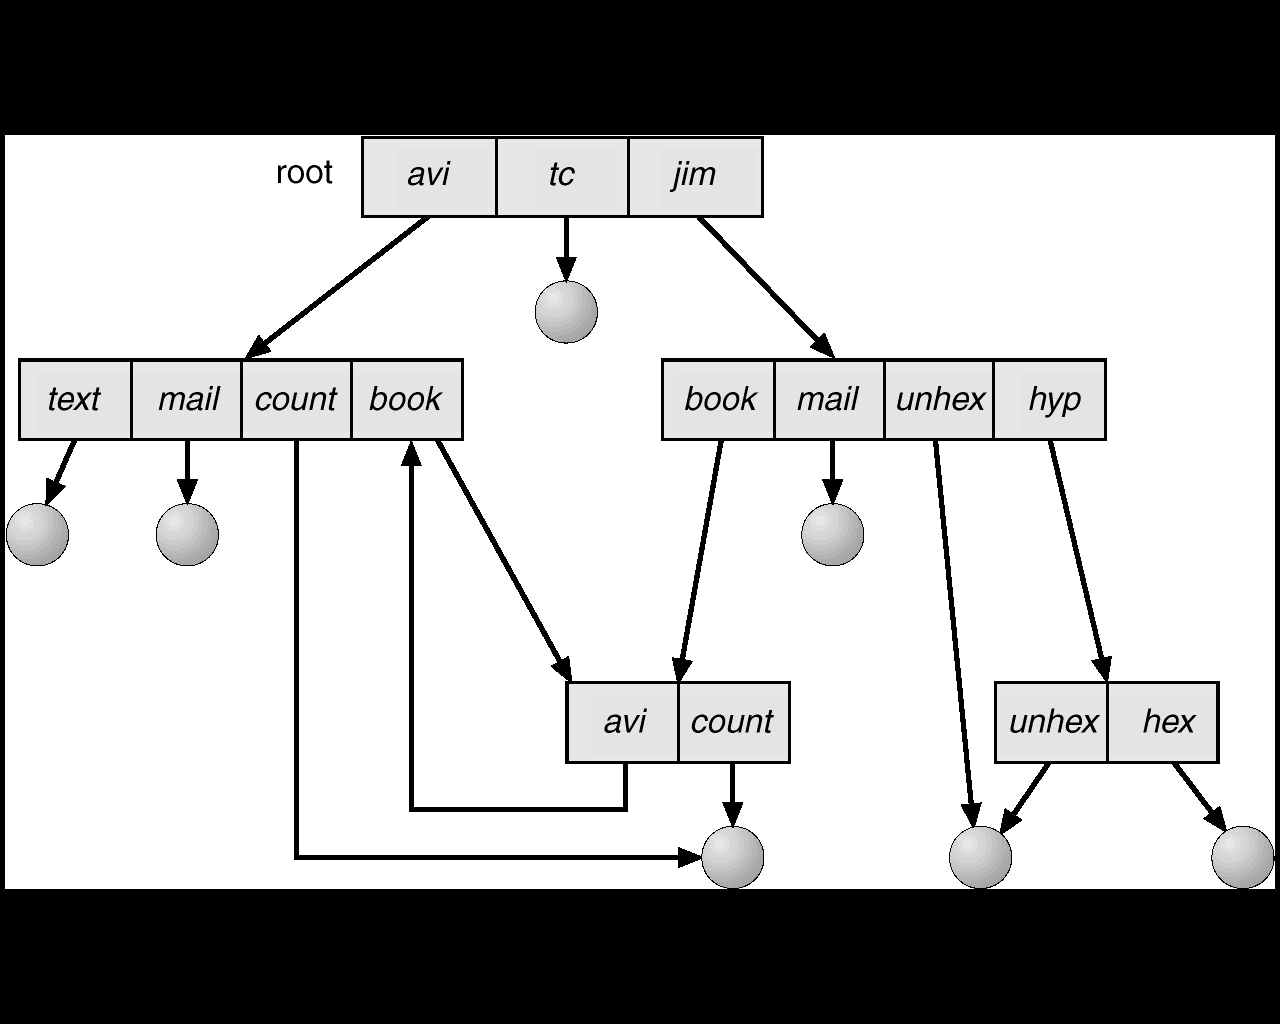
\includegraphics[width=0.50\linewidth]{images/dir_graphGeneralLevel.png} \caption{Directory con struttura a grafo generale} \end{figure}
\nt{
    Per queste ragioni, i sistemi operativi solitamente proibiscono situazioni che portano a cicli nel grafo delle directory.
}

\ex{Strutture a Grafo}{
    Consultare la figura 13.11 per esempi di strutture a grafo generale e per comprendere i limiti imposti dai sistemi operativi.
}

\subsection{Accesso Rapido ai File}
Accedere ad un file attraverso il suo pathname può risultare estremamente inefficiente. Ogni accesso potrebbe richiedere più operazioni sulla Memoria Secondaria, dove file, attributi e directory sono memorizzati.

\ex{Efficienza dell'accesso}{
    Consideriamo un programma che debba scrivere ripetutamente in un file. Se per ogni scrittura fosse necessario specificare la posizione del file nel File System, come nel seguente esempio:
    \begin{verbatim}
    fprintf("/users/john/subdir/myfile", "%d", myvar);
    \end{verbatim}
    tale approccio risulterebbe inefficiente.
}

\wc{
    È importante notare che l'uso di \texttt{fprintf} in questo modo è errato e non è una pratica corretta.
}{
    La corretta gestione dell'accesso ai file prevede l'utilizzo di metodi più efficienti, come l'uso di file descriptor o stream aperti.
}

Quando un programma deve accedere ripetutamente a un file, l'uso diretto del pathname, come nell'esempio di \texttt{fprintf}, risulta estremamente inefficiente. Ogni scrittura richiederebbe di percorrere l'intero pathname, accedendo alla memoria secondaria per ogni directory. Questo comportamento comporta i seguenti passaggi:
\begin{itemize}
    \item Prelevare le informazioni dalla directory radice \(\texttt{/}\) per verificare se contiene la directory \(\texttt{users}\).
    \item Se sì, prelevare dalla memoria secondaria le informazioni della directory \(\texttt{users}\) e verificare se contiene la directory \(\texttt{john}\).
    \item Continuare con questa procedura fino a raggiungere il file \(\texttt{myfile}\).
\end{itemize}

\nt{
    Questo processo risulta inefficiente, poiché richiede molti accessi alla memoria secondaria per recuperare le informazioni di ogni directory.
}

\subsection{Soluzione: Apertura del File}
Per evitare l'inefficienza dell'accesso ai file tramite il loro pathname completo, il sistema operativo richiede ai programmi di aprire i file tramite una system call \texttt{open}. Durante questa apertura, le informazioni relative al file vengono copiate in memoria principale (MP) in una \textit{open file table}.
Dopo l'apertura del file, ogni accesso a tale file avviene attraverso la \textit{open file table} in RAM, anziché passare nuovamente dal filesystem.

\subsection{Esempio di Scrittura su un File}
Un programma che scrive su un file può utilizzare una libreria di I/O come quella di C in Unix, che sfrutta le system call del sistema operativo. Il codice che segue illustra come un programma apre un file, vi scrive e poi lo chiude:

\begin{verbatim}
File *fp;
fp = fopen("/users/john/subdir/myfile", "w");  // apertura del file
fprintf(fp, "%d", myvar);  // scrittura dei dati
fprintf(fp, "%s", "hello");  // scrittura di altri dati
fclose(fp);  // chiusura del file
\end{verbatim}
La system call \texttt{fopen} apre il file e lo associa al puntatore \texttt{fp}, che permette di accedere al file. Le successive operazioni su \texttt{fp} sono gestite in memoria principale.

\subsection{Il Ruolo del "File Pointer"}
Il \texttt{file pointer} \texttt{fp} agisce come una "scorciatoia" per accedere alle informazioni relative al file. Quando il file è aperto tramite \texttt{fopen}, le informazioni sul file vengono copiate nella \textit{open file table} in memoria principale, e \texttt{fp} punta all'entry corrispondente a quel file.

\nt{
    In pratica, \texttt{fp} fornisce un accesso rapido alle informazioni sul file senza dover navigare ripetutamente nel filesystem.
}

\subsection{Cosa Viene Copiato in Memoria Principale durante l'Apertura del File}
Quando un file viene aperto tramite \texttt{open} (o \texttt{fopen}), le informazioni principali del file vengono copiate in memoria principale. Queste informazioni includono, come minimo, tutti gli attributi del file, che vengono letti e aggiornati più velocemente in memoria principale. Inoltre, nel caso di file di grandi dimensioni, anche una porzione del file su cui il processo sta operando può essere copiato in memoria.
Ciò significa che tutte le operazioni sui dati del file vengono eseguite direttamente sulla copia in memoria, migliorando significativamente l'efficienza.

\subsection{Sincronizzazione con la Memoria Secondaria}
Il sistema operativo si occupa di sincronizzare le modifiche effettuate sulla copia in memoria del file con la memoria secondaria. Questo può avvenire periodicamente o, come minimo, quando il file viene chiuso tramite la system call \texttt{close}.

\nt{
    Questo processo garantisce che tutte le modifiche vengano correttamente registrate nel filesystem una volta che il file non è più in uso.
}
